\chapter{Realisierung Objekt Erkennung}\label{kap:object_det}

\section{Datensatz}\label{sec:dataset}

Um ein Deep Learning Modell vernünftig trainieren zu können, 
wird eine große Menge an gelabelten Trainingsdaten benötigt.
Im Falle der Objekterkennung enthalten die labels neben der 
Klasse auch die Koordinaten der Bounding Boxen.


Für die vorliegende Arbeit wurden dafür aus dem Open Source 
Dataset \textit{OpenImages} \cite{kuznetsovaOpenImagesDataset2018} 
von Google 9 Klassen die Wildtiere enthalten heruntergeladen.

Dieses besteht aus einem Trainingsset mit 200 bis 2000 Bildern pro 
Klasse sowie einem Test- und einem Validierungsset. Um für alle Klassen 
die gleiche Anzahl an Trainingsdaten zu erhalten und um Overfitting zu 
verhindern wurden wie im folgenden beschrieben die Trainingsdaten 
augmentiert.

\subsection{Augmentierung}

Augmentierung ist eine Technik aus den vorhandenen Daten 
künstlich mehr Daten zu generieren, indem diese leicht 
abgeändert werden. Im Falle des für diese Arbeit verwendeten
OpenImages Datensatzes wurden Geometrische Transormationen 
wie Sklierung, Verschiebung Rotieren oder Spiegeln und 
Manipulationen der Pixelwerte wie ändern der 
Farbwerte, Helligkeit, Kontrast oder Rauschen vorgenommen.

\begin{figure}[htb]
    \centering
    \label{fig:augmentierung}
    \includegraphics[width=0.8\columnwidth]{Bilder/augmentierung.png}
    \caption{Anwendung von Augmentierungstechniken}
\end{figure}


\section{Training}

Da der Neural Compute Stick mit OpenVino ein eigenes Datei Format 
für die traininerten Modelle verwendet, musste bei der Auswahl
eines Frameworks sowie Models auf die Kompatibilität zu OpenVino 
geachtet werden. 

Verwendete wurde daher das untersstütze Framework Tensorflow, 
um zwei Ansätze zu verfolgen. Der eine verwendet die Api Keras, 
und versucht neben der Klassifikation die Lokalisierung mit 
dieser vorzunahemen, der andere verwendet eine speziell für die 
Objekterkennung konzipierte Api für wie in Abschnitt
 \ref{sec:related_work} beschriebene End-to-End lösungen.

\subsection{Tensorflow Object Detection Api}

Die Tensorflow Object Detection Api ist unter den Research Modellen
\cite{HttpsGithubCom} des offiziellen Tensorflow Repository zu
finden und enthällt implementierungen einiger gängiger Object Detectin
Modelle, wie Single Shot Detectors (SSD) und Faster R-CNNs mit 
verschiedenen Basis CNNs mit vortrainierten Geweichten.

Um die Modelle trainieren zu können, mussten zunächst die 
Trainingsdaten in das binary Dateiformate TFRecords umgewandelt 
werden, welches die Api verwendet. Dieses ist eine Serialisierte 
darstellung der Bilder und Labels als Protocol Buffer für
effizienten Zugriff auf diese.

Trainiert wurde mit hilfe \textit{Google Colab}, eine cloudbasierte VM,
welche eine \dots Gpu zur verfügung stellt.

\subsection{Trainingsoptimierung}

Um zu einem guten Ergebnis zu kommen werden, wie in ... dargestellt, 
häufig Anpassung bezogen auf Datensatz Augmentierungstechniken, 
verschiedene Modell und Basis CNNs, sowie dessen Hyperparameter vorgenommen.

\begin{figure}[htb]
    \centering
    \def\svgwidth{0.7\textwidth}
    
\tikzstyle{process} = [rectangle, fill=blue!20, node distance=4cm, minimum width=1.5cm, minimum height=0.8cm, text centered, draw=black]
\tikzstyle{arrow} = [thick,->,>=stealth]
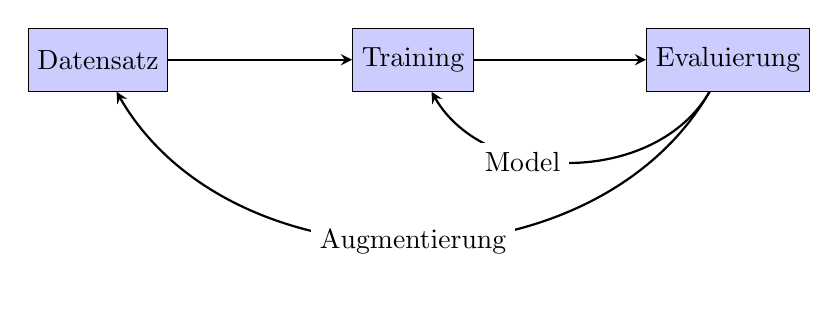
\begin{tikzpicture}[scale=0.4]
      \node (data)      [process]                   {Datensatz};
      \node (train)      [process, right of=data]      {Training};
      \node (eval)      [process, right of=train]      {Evaluierung};
    \draw[arrow] (data) -- (train);
    \draw[arrow] (train) -- (eval);
  \draw[arrow] (eval) edge[bend left=60] node [centered, fill=white!30] {Augmentierung} (data);
  \draw[arrow] (eval) edge[bend left=60] node [left, fill=white!30] {Model} (train);
\end{tikzpicture}

% \begin{tikzpicture}[scale=0.4]

%   \begin{scope}[node distance=3cm]

%    \node (data)      [process]                   {Datensatz};
%    \node (prep)      [process, right of=data]      {Aufbereitung};
%    \node (model)      [process, right of=prep]      {Model};
%    \node (train)      [process, right of=model]      {Training};
%    \node (eval)      [process, right of=train]      {Evaluierung};

%   \end{scope}

%  \draw[arrow] (data) -- (prep);
%  \draw[arrow] (prep) -- (model);
%  \draw[arrow] (model) -- (train);
%  \draw[arrow] (train) -- (eval);
 

% \draw[arrow] (eval) edge[bend left=60] node [left, fill=white!30] {ändern} (data);
% \draw[arrow] (eval) edge[bend left=60] node [left, fill=white!30] {augment} (prep);
% \draw[arrow] (eval) edge[bend left=60] node [left, fill=white!30] {ändern} (model);
% \draw[arrow] (eval) edge[bend left=60] node [left, fill=white!30] {Parameter} (train);

 
% \end{tikzpicture}

    \caption{Trainingsworkflow}
    \label{fig:train_workflow}
\end{figure}

\begin{itemize}
    \item Datensatz
    \begin{itemize}
        \item Augmentierungstechniken
        \begin{itemize}
            \item Geometrische
            \item Farbwerte
        \end{itemize}
        \item Graustufen
        \begin{itemize}
            \item 1 Channel
            \item 3 Channel
        \end{itemize}
    \end{itemize}
    \item Modelle
    \begin{itemize}
        \item Faster R-CNNs
        \begin{itemize}
            \item InceptionV2
            \item Resnet
        \end{itemize}
        \item SSD
        \begin{itemize}
            \item Mobilenet
            \item InceptionV2
        \end{itemize}
    \end{itemize}
    \item Hyperparameter
    \begin{itemize}
        \item Dropout
        \item L2 Realisierung
        \item Early Stopping
    \end{itemize}
\end{itemize}



